\subsection{Formal Languages and Grammars}
\label{subsec:formal-languages-and-grammars}


The study of automata begins with the fundamental concepts of formal language theory, a field that emerged from the pioneering work of Stephen Kleene, Noam Chomsky, Alan Turing, and Michael Rabin. Kleene's early work on the representation of events in nerve nets and finite automata \cite{kleene1956representation} laid the groundwork for understanding the algebraic structure of languages. Chomsky’s introduction of language hierarchies \cite{chomsky1956three} further clarified how different classes of languages can be recognised by increasingly powerful computational models. Turing's conceptualization of computation \cite{hopcroft2006introduction} provided a model for algorithmic processes, while Rabin's introduction of probabilistic automata \cite{rabin1963probabilistic} expanded the framework to include models where transitions are governed by probability. 

These seminal contributions collectively established the mathematical scaffolding for the study of automata and formal languages. Their rigorous definitions and operations are not only abstract mathematical constructs; they serve as the basis for practical applications. For example, regular expressions—rooted in the theory of regular languages—are widely used in text processing and programming language design. Similarly, the limitations of context-free languages have led to the development of more advanced parsing techniques in compilers.



\begin{notation}[Symbols]
In this thesis, the following notations are used:
\begin{itemize}
    \item $\Sigma$: an alphabet, i.e., a non-empty finite set of symbols.
    \item $\Sigma^\ast$: the Kleene closure of $\Sigma$, the set of all finite strings over $\Sigma$.
    \item $\epsilon$: the empty string (with $\|\epsilon\| = 0$).
    \item $\|w\|$: the length of a string $w$.
\end{itemize}
\end{notation}

\subsubsection{Alphabets and Strings}
An \textit{alphabet} $\Sigma$ is defined as a non-empty, finite set of symbols that serve as the basic elements for constructing strings and, consequently, languages. For instance:

\begin{example}
\textbf{Binary Alphabet:} $\Sigma = \{0, 1\}$ is central to digital computing and coding theory \cite{hopcroft2006introduction}.
\end{example}

\begin{example}
\textbf{ASCII Alphabet:} $\Sigma_{\text{ASCII}}$, which contains 128 distinct characters used for text encoding \cite{cady1986ascii}.
\end{example}

A \textit{string} (or \textit{word}) $w$ over $\Sigma$ is a finite sequence of symbols $a_1a_2\ldots a_n$, where each $a_i \in \Sigma$. The \textbf{length} of $w$, denoted by $\|w\|$, is defined as the total number of symbols in the string. The special string $\epsilon$, known as the \textbf{empty string}, has a length of zero ($\|\epsilon\| = 0$) \cite{hopcroft2006introduction}.

\begin{example}
For $\Sigma = \{a, b\}$, consider the string $w = aba$. Then, $\|w\| = 3$. Conversely, $w = \epsilon$ represents the absence of input.
\end{example}

\begin{remark}
The concepts of $\Sigma$, $\Sigma^\ast$, and $\epsilon$ form the foundation for all language constructions and are pivotal when defining operations such as concatenation and the Kleene star.
\end{remark}

In addition to defining strings, several operations are essential for manipulating them:
\begin{itemize}
    \item \textbf{Reversal}: The operation $w^R$ produces the string obtained by reversing the order of symbols in $w$ (e.g., $(abc)^R = cba$) \cite{hopcroft2006introduction}.
    \item \textbf{Substring}: A string $v$ is a substring of $w$ if there exist (possibly empty) strings $x$ and $y$ such that $w = xvy$ \cite{hopcroft2006introduction}.
\end{itemize}

\subsubsection{Languages and Operations}
A \textit{language} $L$ is a subset of $\Sigma^\ast$, where $\Sigma^\ast$ denotes the \textbf{Kleene closure} of $\Sigma$, defined as:
\[
\Sigma^\ast = \bigcup_{n=0}^\infty \Sigma^n, \quad \text{where } \Sigma^0 = \{\epsilon\}.
\]
\cite{kleene1956representation}

Languages are constructed and manipulated using various operations. These operations are central to proofs of language properties and decidability:

\begin{enumerate}
    \item \textbf{Concatenation}: For two languages $L_1$ and $L_2$, their concatenation is defined by 
    \[
    L_1 \cdot L_2 = \{xy \mid x \in L_1,\, y \in L_2\}.
    \]
    \begin{example}
    Let $L_1 = \{a, ab\}$ and $L_2 = \{b, ba\}$. Then,
    \[
    L_1 \cdot L_2 = \{ab, aba, abb, abba\},
    \]
    which demonstrates the formation of new languages by joining strings from different languages \cite{hopcroft2006introduction}.
    \end{example}

    \item \textbf{Union/Intersection}: These operations are defined as:
    \begin{align*}
        L_1 \cup L_2 &= \{w \mid w \in L_1 \text{ or } w \in L_2\}, \\
        L_1 \cap L_2 &= \{w \mid w \in L_1 \text{ and } w \in L_2\}.
    \end{align*}
    They allow the combination or filtering of languages based on shared elements \cite{hopcroft2006introduction}.

    \item \textbf{Kleene Star}: The Kleene star operation generates the set of all possible concatenations (including the empty string) of elements from a language:
    \[
    L^\ast = \bigcup_{i=0}^\infty L^i, \quad \text{where } L^i = \underbrace{L \cdot L \cdots L}_{i \text{ times}}.
    \]
    \begin{example}
    For $L = \{0, 1\}$, the set $L^\ast$ comprises all binary strings, including $\epsilon$ \cite{hopcroft2006introduction}.
    \end{example}

    \item \textbf{Complement}: The complement of a language $L$ with respect to $\Sigma^\ast$ is defined as 
    \[
    \overline{L} = \Sigma^\ast \setminus L.
    \]
    This operation is useful for expressing languages indirectly \cite{hopcroft2006introduction}.

    \item \textbf{Homomorphism}: A homomorphism is a function $h: \Sigma^\ast \to \Gamma^\ast$ that maps each symbol in $\Sigma$ to a string in $\Gamma^\ast$. For example, if $h(a) = 01$, then every occurrence of $a$ in a string is replaced by $01$ \cite{hopcroft2006introduction}.

    \item \textbf{Inverse Homomorphism}: Given a homomorphism $h$, the inverse homomorphism is defined by 
    \[
    h^{-1}(L) = \{w \mid h(w) \in L\},
    \]
    which retrieves the pre-images from the target language \cite{hopcroft2006introduction}.
\end{enumerate}

\subsubsection{Language Categories}
Languages are classified according to the type of automata that recognise them and their inherent structural complexity. The main categories are as follows:

\begin{enumerate}
    \item \textbf{\glspl{reg}}:  
    These languages are recognised by \gls{dfa} and \gls{nfa} and can be generated by regular expressions \cite{hopcroft2006introduction}. 
    \begin{example}
    $L = \{w \in \{a, b\}^\ast \mid w \text{ contains } aba\}$ is a regular language \cite{hopcroft2006introduction}.
    \end{example}
    
    \item \textbf{\glspl{cfl}}:  
    These languages are recognised by \gls{pda} and generated by context-free grammars \cite{chomsky1956three, hopcroft2006introduction}.  
    \begin{example}
    $L_{\text{pal}} = \{ww^R \mid w \in \{a, b\}^\ast\}$, the language of palindromes, is a classic example \cite{chomsky1956three}.
    \end{example}

    \item \textbf{\glspl{csl}}:  
    Recognised by linear-bounded automata, these languages have structural constraints that extend beyond context-free languages \cite{chomsky1956three, hopcroft2006introduction}.  
    \begin{example}
    $L = \{a^n b^n c^n \mid n \geq 1\}$ is an example of a context-sensitive language \cite{chomsky1956three}.
    \end{example}

    \item \textbf{Recursively Enumerable Languages (Type-0)}:  
    Recognised by \glspl{tm}, these languages embody the notion of algorithmic computability \cite{hopcroft2006introduction, turing1936computable}.  
    \begin{example}
    The language corresponding to the Halting Problem is recursively enumerable \cite{hopcroft2006introduction}.
    \end{example}

    \item \textbf{Stochastic Languages}:  
    Recognised by \glspl{pfa} with bounded error, stochastic languages allow for probabilistic acceptance criteria \cite{rabin1963probabilistic}.  
    \begin{example}
    $L_{\text{eq}} = \{a^n b^n \mid n \geq 1\}$ is stochastic but not regular. A \gls{pfa} can accept it with probability at least $\frac{2}{3}$ for strings in $L_{\text{eq}}$ and at most $\frac{1}{3}$ for strings not in $L_{\text{eq}}$ \cite{rabin1963probabilistic}.
    \end{example}
\end{enumerate}

\begin{definition}[Regular Language]
A language $L \subseteq \Sigma^\ast$ is \textit{regular} if there exists a \gls{dfa} (or an equivalent \gls{nfa}) that accepts exactly the strings in $L$.
\end{definition}

\begin{theorem}[Pumping Lemma for Regular Languages]
\label{thm:pumping-lemma}
Let $L \subseteq \Sigma^\ast$ be a regular language. Then there exists an integer $p \geq 1$, known as the \textit{pumping length}, such that every string $s \in L$ with $\|s\| \geq p$ can be decomposed into three parts $s = xyz$, satisfying:
\begin{enumerate}
    \item $|xy| \leq p$,
    \item $|y| \geq 1$, and
    \item For all $i \geq 0$, the string $xy^iz \in L$.
\end{enumerate}
\end{theorem}

\begin{corollary}
If a language $L$ fails to satisfy the conditions of Theorem~\ref{thm:pumping-lemma} for any possible pumping length $p$, then $L$ is not regular.
\end{corollary}

\subsubsection{Closure Properties}
Closure properties determine how language classes behave under various operations—a critical aspect in proving decidability and constructing new languages:

\begin{itemize}
    \item \textbf{\glspl{reg}}: closed under union, intersection, complement, concatenation, and Kleene star \cite{hopcroft2006introduction}.
    \item \textbf{\glspl{cfl}}: closed under union and Kleene star, but not under intersection or complement \cite{chomsky1956three, hopcroft2006introduction}.
    \item \textbf{\glspl{csl}}: closed under union, intersection, and complement \cite{chomsky1956three, hopcroft2006introduction}.
    \item \textbf{Stochastic Languages}: closed under union, intersection, and concatenation, but not under complementation or Kleene star \cite{rabin1963probabilistic, paz1971introduction}.
\end{itemize}

\begin{observation}
Closure properties not only simplify the construction of new languages from known ones but also play a key role in proving undecidability results. For instance, the non-closure of context-free languages under intersection and complementation is a cornerstone in many undecidability proofs.
\end{observation}

\begin{example}
The closure of regular languages under intersection guarantees that if $L_1, L_2 \in \glspl{dfa}$ (or, equivalently, recognised by \glspl{nfa}) then $L_1 \cap L_2$ is also regular. In contrast, although stochastic languages are closed under intersection, they are not closed under complementation, as demonstrated by the inability to recognise 
\[
\overline{L_{\text{eq}}} \quad \text{for} \quad L_{\text{eq}} = \{a^n b^n \mid n \geq 1\}
\]
\cite{rabin1963probabilistic}.
\end{example}

\begin{table}[h]
    \centering
    \begin{adjustbox}{max width=\textwidth}
    \begin{tabular}{@{}lccccc@{}}
        \toprule
        \textbf{Operation} & \glspl{reg} & \glspl{cfl} & \glspl{csl} & Stochastic & Type-0 \\ \midrule
        Union          & \checkmark & \checkmark & \checkmark & \checkmark & \checkmark \\
        Intersection   & \checkmark & $\times$ & \checkmark & \checkmark & \checkmark \\
        Complement     & \checkmark & $\times$ & \checkmark & $\times$ & \checkmark \\
        Concatenation  & \checkmark & \checkmark & \checkmark & \checkmark & \checkmark \\
        Kleene Star    & \checkmark & \checkmark & \checkmark & $\times$ & \checkmark \\ \bottomrule
    \end{tabular}
    \end{adjustbox}
    \caption{Comparison of closure properties for different language classes}
    \label{tab:closure-properties}
\end{table}

\subsubsection{Chomsky Hierarchy}
Formal languages are organised into a hierarchical framework known as the Chomsky hierarchy \cite{chomsky1956three, hopcroft2006introduction}:
\begin{enumerate}
    \item \textbf{Type-3 (Regular)}: Languages recognised by \glspl{dfa} (or \glspl{nfa}) \cite{hopcroft2006introduction}.
    \item \textbf{Type-2 (Context-Free)}: Languages recognised by \glspl{pda} \cite{chomsky1956three}.
    \item \textbf{Type-1 (Context-Sensitive)}: Languages recognised by linear-bounded automata \cite{chomsky1956three}.
    \item \textbf{Type-0 (Recursively Enumerable)}: Languages recognised by \glspl{tm}, which formalise the notion of algorithmic computability \cite{hopcroft2006introduction, turing1936computable}.
\end{enumerate}

\begin{concept}
The Chomsky hierarchy not only classifies languages based on the computational power needed for recognition but also reflects the trade-offs between expressiveness and computational complexity.
\end{concept}

\begin{figure}[h]
    \centering
    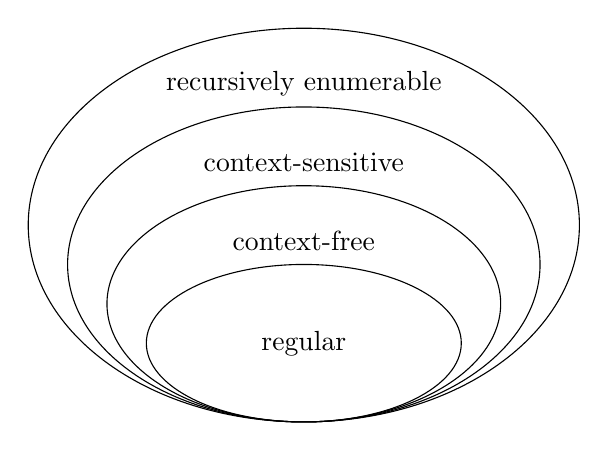
\begin{tikzpicture}
        \draw (0,0) ellipse (2 and 1);
        \draw (0,0.5) ellipse (2.5 and 1.5);
        \draw (0,1) ellipse (3 and 2);
        \draw (0,1.5) ellipse (3.5 and 2.5);
        \node at (0,0) {regular};
        \node at (0,1.3) {context-free};
        \node at (0,2.3) {context-sensitive};
        \node at (0,3.3) {recursively enumerable};
    \end{tikzpicture}
    \caption{Chomsky hierarchy of formal languages}
    \label{fig:chomsky-hierarchy}
\end{figure}

\subsubsection{Practical Implications}
The theoretical constructs discussed above are not only of academic interest but also have significant practical applications:
\begin{itemize}
    \item \textbf{Regular Expressions}: Extensively used in text processing (e.g., in tools such as \texttt{grep} and in lexical analysers) \cite{kernighan1984unix, hopcroft2006introduction}.
    \item \textbf{Context-Free Grammars}: Form the basis for defining the syntax of programming languages such as Python and Java \cite{chomsky1956three, hopcroft2006introduction}.
    \item \textbf{Closure Properties}: Provide a framework for proving decidability results (e.g., the emptiness problem for \glspl{dfa}) \cite{hopcroft2006introduction}.
    \item \textbf{Stochastic Models}: Are applied in areas like natural language processing and speech recognition, where probabilistic pattern matching is essential \cite{rabin1963probabilistic}.
\end{itemize}